% Created 2022-03-21 Mon 12:43
% Intended LaTeX compiler: pdflatex
\documentclass{IEEEtran}
\usepackage[utf8]{inputenc}
\usepackage[T1]{fontenc}
\usepackage{graphicx}
\usepackage{longtable}
\usepackage{wrapfig}
\usepackage{rotating}
\usepackage[normalem]{ulem}
\usepackage{amsmath}
\usepackage{amssymb}
\usepackage{capt-of}
\usepackage{hyperref}
\usepackage[backend=biber, style=numeric]{biblatex}

\addbibresource{reference.bib}
\author{Anak Wannaphaschaiyong}
\date{\textit{<2022-03-03 Thu>}}
\title{Ensemble Approaches for Streaming Networking Classification}
\begin{document}

\maketitle

\section{Introduction}
\label{sec:orgdb6452b}
Dynamic graph is a vaguely used term. In general, dynamic graph is an ordered list of node and link events. These events include deletion and addition of nodes and edges after a interval of time.
Dynamic graph is known in other named as streaming graph and temporal graph. Concretely, dynamic graph can be categorized into taxonomies. A few embedding dynamic network surveys have attempted to provide these taxonomies \cite{barrosSurveyEmbeddingDynamic2021,kazemiRepresentationLearningDynamica,skardingFoundationsModelingDynamic2021}.

In static network, one must consider type of network relationship (e.g idealize network, proximity network.), scale of network (e.g. a node as a single entity, a node as a group of entities.), and network variation (e.g. homogenous network, heterogenous network, multilayer network).
The mentioned factors provide unique challenges. These factors must be considered before model designing phase starts otherwise network based models cannot be compared fairly. Moreover, it provide mental framework to guide designing process.

Dynamic graph extends static graph to include time variables. This add more degree of freedom to the problem. Additional degree of freedom include network status (how is information about network aggregated over time.), dynamic behavior on graph (communication behavior between nodes) and graph evolution. (structure,features,role evolution of a graph.)

Currently, in the field of machine learning on dynamic network, simply train-test split is used to conclude models performance. This is not a good idea because dynamic network data is a sequential data. It is more appropriate to use sliding window evaluation. Sliding window evaluation is a well known technique that is a gold standard for sequential data such as time series data. Furthermore, we found that models capacity directly depends on sliding window parameters such as window size, epoch per window etc. Therefore, without adopting sliding window evaluation as a standard to evaluate performance of dynamic network, one cannot create a fair environment to compare performance between dynamic network based models.
For this reason, in this paper, we adopt window sliding window evaluation to evaluate link prediction and node classification using dynamic network as input.
The paper analyze multiple ensemble approaches which can only be adopted via sliding window evaluation. This provides another tool to be used within dynamic graph environment.

[What are brief results of the proposed design?] It is not yet clear to me what I should write for this.

\section{Related Work}
\label{sec:orgfcba84c}
\subsection{Dynamic Graph}
\label{sec:orgd82ad8e}
\subsubsection{Taxonomies of Dynamic Graph}
\label{taxonomies of dynamic graph}
At the time of writing many taxonomies of dynamic graph models has been proposed.
In this related work section, we will discuss previous attempts to categorize dynamic graph models into groups. Before discussing previous attempt, one should understand types of dynamic behavior that can affect dynamic graph models. There are two types of dynamic behaviors which are referred to in referenced literature by different names, nonetheless, we will refer to the two types as ``dynamic behavior on graph'' and ``dynamic behavior over graph''. One can think of dynamic behavior on graph as communication between nodes that happens via edges. Dynamic  behavior over graph can be think of as changes of graph as a whole over time. Intuitively, ``dynamic behavior on graph'' concerns micro (node/edges) levels while ``dynamic behavior over graph'' concern macro level --- concern graph as a whole. An example to emphasize on the difference, given that there exist a group of individuals, Evolution of individuals (nodes) ``role'' depends on when and how they interact. At the macro level, a member of a group may leave and join. This behavior also depends on time interval that experiment considers.

Furthermore, design of models directly depend on dynamic behavior involved in dynamic graph. Hence, due to the factor mentioned above, it is very important to create an environment that is fair to make comparison between dynamic graph models. In addition to factor mentioned above, there are other factors that directly influence behavior on/over a graph including size of graph, node scale, et cetera, which beyond the scope of the paper. Empirical experiment has shown that combination of factors previously mentioned produces different temporal characteristic of dynamic graph either on/over the graph e.g. business property \cite{holme2012temporal} among other.

Barros et al. \cite{barrosSurveyEmbeddingDynamic2021} categorized dynamic graph based on output embedding, model approaches, and dynamic behavior over graph. On the other than, Kazemi et al. \cite{kazemiRepresentationLearningDynamica} discuss in-depth mathematical formulation of encoder-decoder, one of many model approaches. The discussion also cover other types of models that are more specialized such as dynamic knowledge graph and spatio-temporal graph.

Skarding et al. \cite{skardingFoundationsModelingDynamic2021} takes interesting approach to categorized dynamic graph based on edges duration into interaction networks, temporal networks, evolving networks, and strictly evolving networks. Futhermore, the paper classifies dynamic network models into statical models, stochastic actor oretied models, and dynamic network representation learning model. In comparison, Skarding et al. \cite{skardingFoundationsModelingDynamic2021} and Kazemi et al. \cite{kazemiRepresentationLearningDynamica} provides two different ways to categorize dynamic graph models. In contrast to Kazemi et al, Skarding et al. focus mainly on taxonomies of dynamic graph neural network including pseudo-dynamic model, edge-weighted model, discrete model, continuous models.

Note that meaning of temporal networks is ambiguous outside of skarding et al's paper \cite{skardingFoundationsModelingDynamic2021} context. In ``Temporal Network'' paper, Holme et al. \cite{holme2012temporal} introduce ``time-respecting'' path as a property of temporal network. Graph with time-respect path contains edges whose weight value represents time when edges forms. We will adopt taxonomy presented in \cite{skardingFoundationsModelingDynamic2021} because including adopting temporal network definition. This is unambiguous because time-respecting path has not explored at all in the machine learning at the time of writing. Furthermore, all types of dynamic graph can be represented as a form of multilayer graph. \cite{kivela2014multilayer}


\subsubsection{Dynamic Graph Modeling}
\label{sec:orgaacc894}
TGN,
\subsection{Sliding Window Evaluation}
\label{sec:org03541a5}
Sliding window is the basis of how to turn any time series dataset into a supervised learning problem. Given that an instance in a dataset is a event with timestamp, train-test-split are a kind of sliding window where you only have 1 window to train to predict the future. Because temporal properties of time window depends on window size and interval of time, evaluate performance based on sliding window show model's performance under various temporal condition, hence, performance of models cannot be manipulated.

Sliding window is specially important in dynamic based graph when applying ensemble models on top of dynamic graph models, as we will show later, overall performance depends on size of window, number of epoch per window, number of windows, number of batch per window, number of window, and time budget.

Furthermore, sequence of windows allows one to apply a higher level of abstraction over sequence of events which may influence models design. In this case, sliding window evaluation must be applied to all the models involve to create a fair comparison.

In the time of writing, dynamic graph model literature still uses simple train-val-test split as a model evaluation standards. We provide examples of well accepted paper to make a point. Tian et al. \cite{tian2021self} use 70-15-15 split to evaluate self-supervised learning on strictly evolving graph and compare with models. Performance of models are evaluated based on two tasks: link prediction and node classification. The comparison is limited to static graph models, and dynamic random walk. Details to extend static graph models to dynamic graphs are not discussed. Similarly, using the same dataset, Rossi et al. \cite{rossi2020temporal} also use 70-15-15 splits. Rossi et al. compare its own, temporal graph neural network (TGN) to one other dynamic graph, DyRep. The comparison is acceptable because same dataset is used in the experiment. Dataset used in mentioned papers are collected as undirected interaction network.

It is very important to understand that how models receive data --- stream data, one instance at a time, or in batch --- implies underlying graph type. This is because it implies existence duration of nodes and edges which is used to classify dynamic graph based on taxonomies proposed by Skarding et al. \cite{skardingFoundationsModelingDynamic2021}. For detail about taxonomies of dynamic graph can be found in \ref{taxonomies of dynamic graph} section.

To the best of my knowledge, Skarding et al. wrote ``BENCHMARKING GRAPH NEURAL NETWORKS ON DYNAMIC LINK PREDICTION'' \cite{skarding2021benchmarking} which is the only paper to compare dynamic network based models using sliding window evaluation. Directed and undirected interaction network is used. Interaction network can be easily aggregated to form ``graph snapshot.'' Hence, using interaction network, one can pass in continuous network to continuous model and discrete network to discrete models.

Performance of each model varies across metric score. Hence, the paper concludes that optimizing the hyperparamters is essential for obtaining a representative score. This conclusion applies for both static and dynamic graph models. Furthermore, Skarding et al. observes that using window of size 5 or 10 consistently produce best results particularly among discrete models.
\section{Dataset}
\label{sec:org3e2401e}
\textbf{Reddit dataset}: Reddit dataset are a bipartite network of interaction network involving two groups of nodes: Reddit threads and users. Row of the dataset is a tuple of including user-id, thread-id, timestamp, whether user is banned after this event, and pre-compute embedding score with 172 dimensions. There are 672448 instances of interaction (aka edges) which is collected in one month time interval with total 11,000 nodes. Property of Reddit dataset is shown in Table \ref{Datasets}.

\begin{table}[htbp]
\caption{\label{Datasets}Datasets}
\centering
\begin{tabular}{ll}
\hline
\hline
 & Reddit\\
\hline
\# Nodes & 11,000\\
\# Edges & 672,447\\
\# Edges Features & 172\\
Timestapn & 1 month\\
positive label percentages & 0.05 \%\\
\end{tabular}
\end{table}
\section{Approaches}
\label{sec:orga6314fc}
\begin{table}[htbp]
\caption{\label{parameters}Parameters symbols and descriptions}
\centering
\begin{tabular}{lll}
\hline
\hline
 & parameters & description\\
\hline
window parameters & \(w_i\) & i-th window\\
 & \(ws\) & window size\\
 & \(\vert w \vert\) & number of window used during training\\
 & \(bs\) & batch size for a given window where \(bs < ws\)\\
temporal parameters & \(stride\) & window stride\\
 & \(pred\_next_{n}\) & predict instances that are in window that is n window away.\\
 & \(keep\_last\_n\) & number of window to keep as window slides forward\\
 & \(total\_training_windows\) & total number of instances to be trained for\\
ensemble parameters & \(E_i\) & i-th model in ensemble\\
 & \(\vert E \vert\) & number of models used in ensemble\\
 & \(\vert train\_w_{i} \vert\) & i-th window is the first window to begin training\\
granularity parameters & \(PW\) & granularity of prediction. Prediction length during training\\
\end{tabular}
\end{table}

\begin{figure}[htbp]
\centering
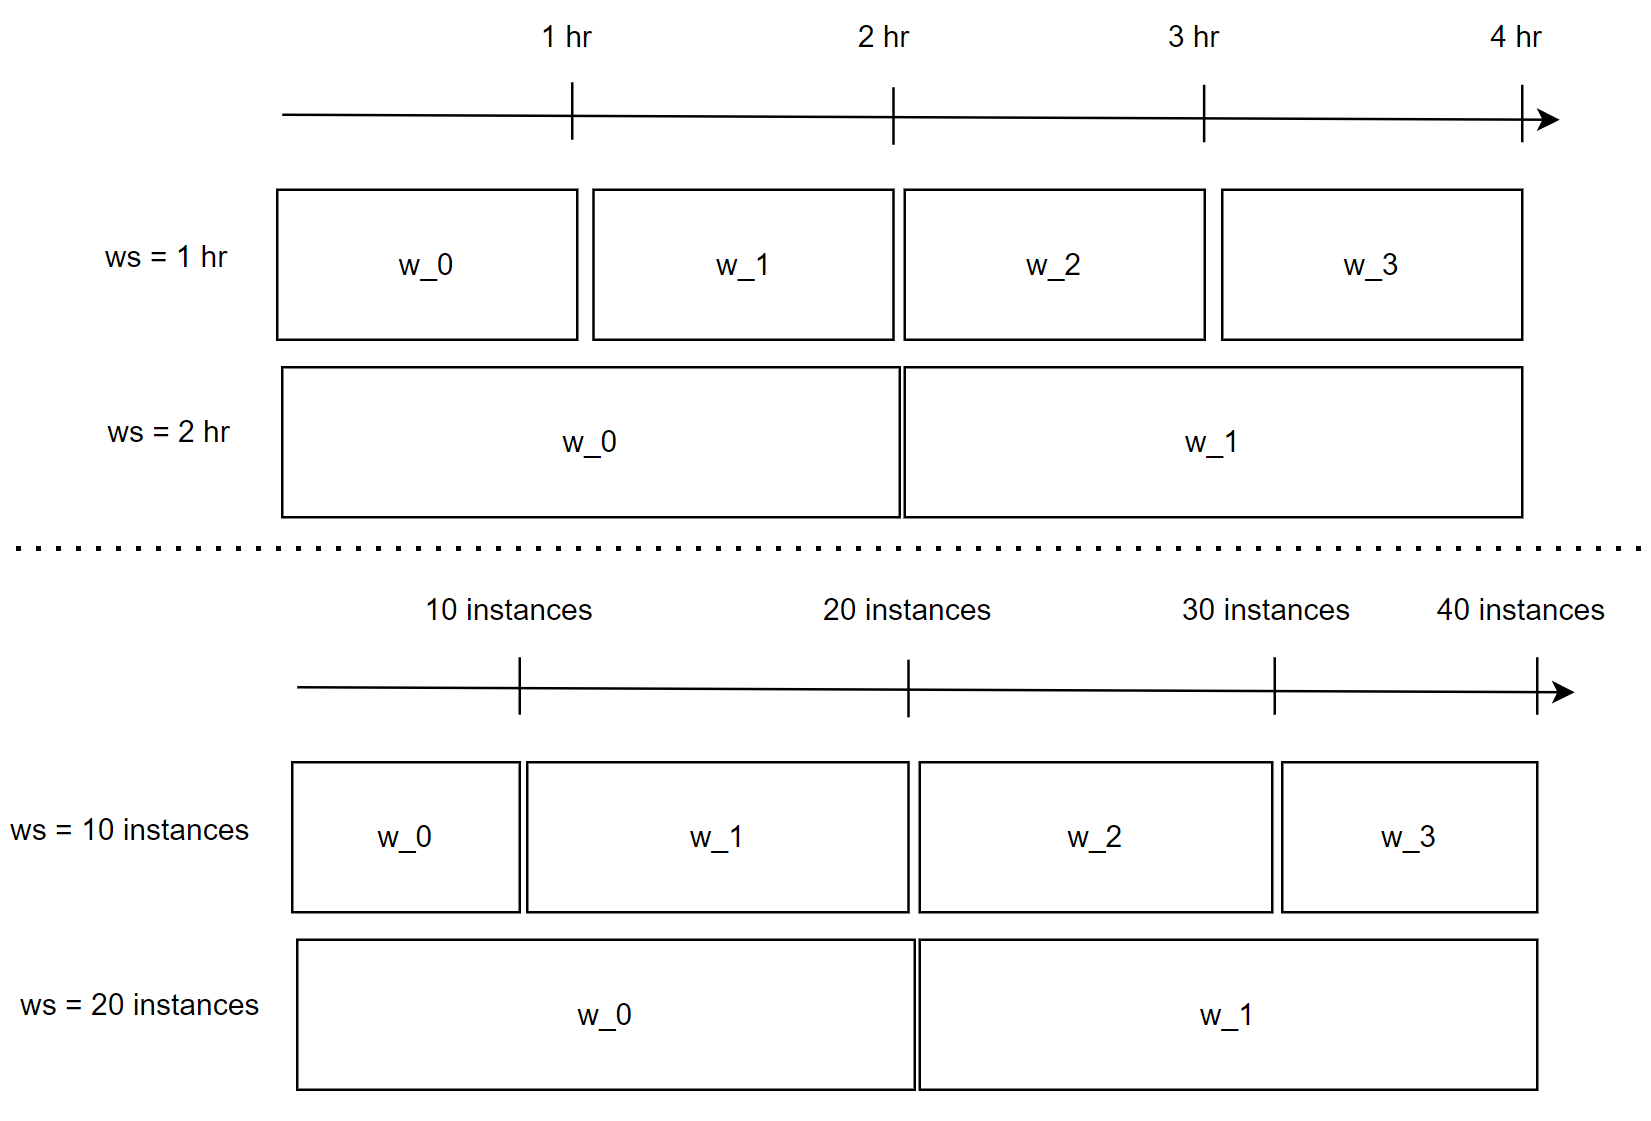
\includegraphics[width=.9\linewidth]{./images/screenshot_20220321_110302.png}
\caption{\label{window parameters}window parameters}
\end{figure}

\begin{figure}[htbp]
\centering
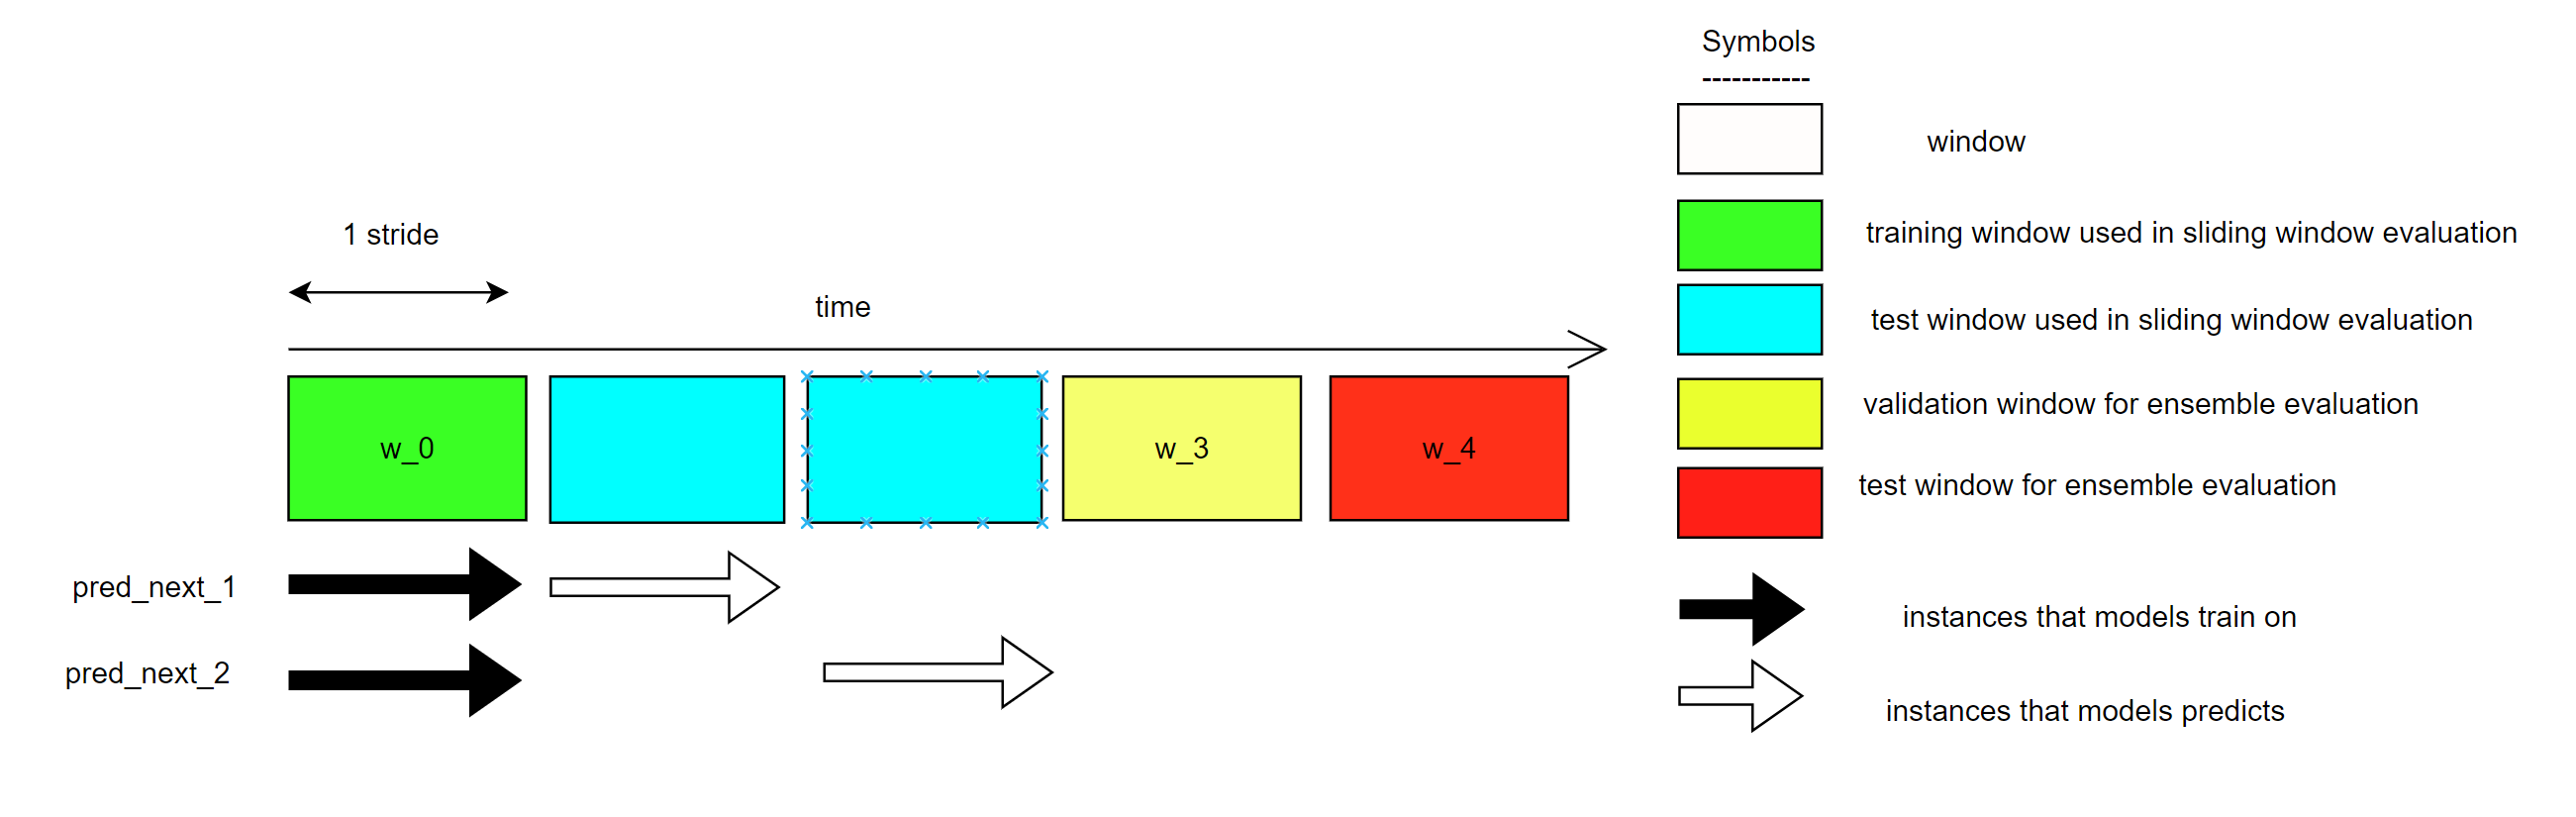
\includegraphics[width=.9\linewidth]{./images/screenshot_20220321_120616.png}
\caption{\label{window parameters}temporal parameters}
\end{figure}

\begin{figure}[htbp]
\centering
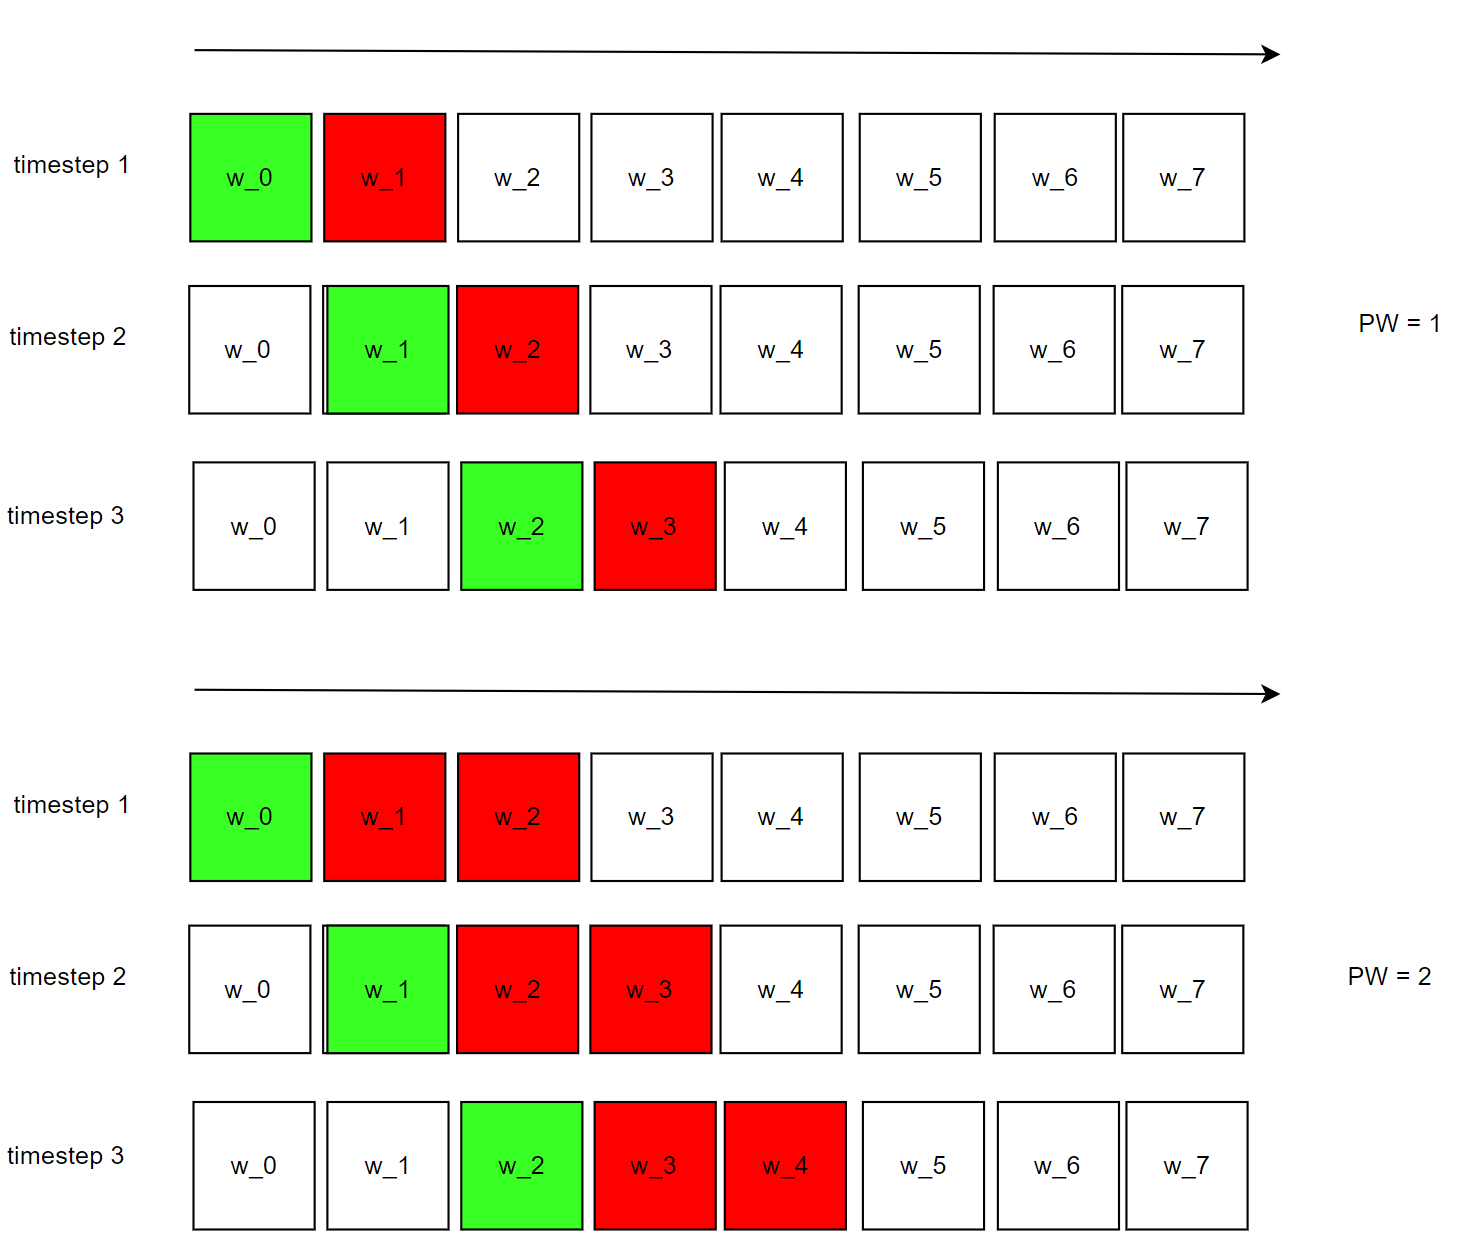
\includegraphics[width=.9\linewidth]{./images/screenshot_20220321_121434.png}
\caption{\label{window parameters}granularity parameters}
\end{figure}

\begin{figure}[htbp]
\centering
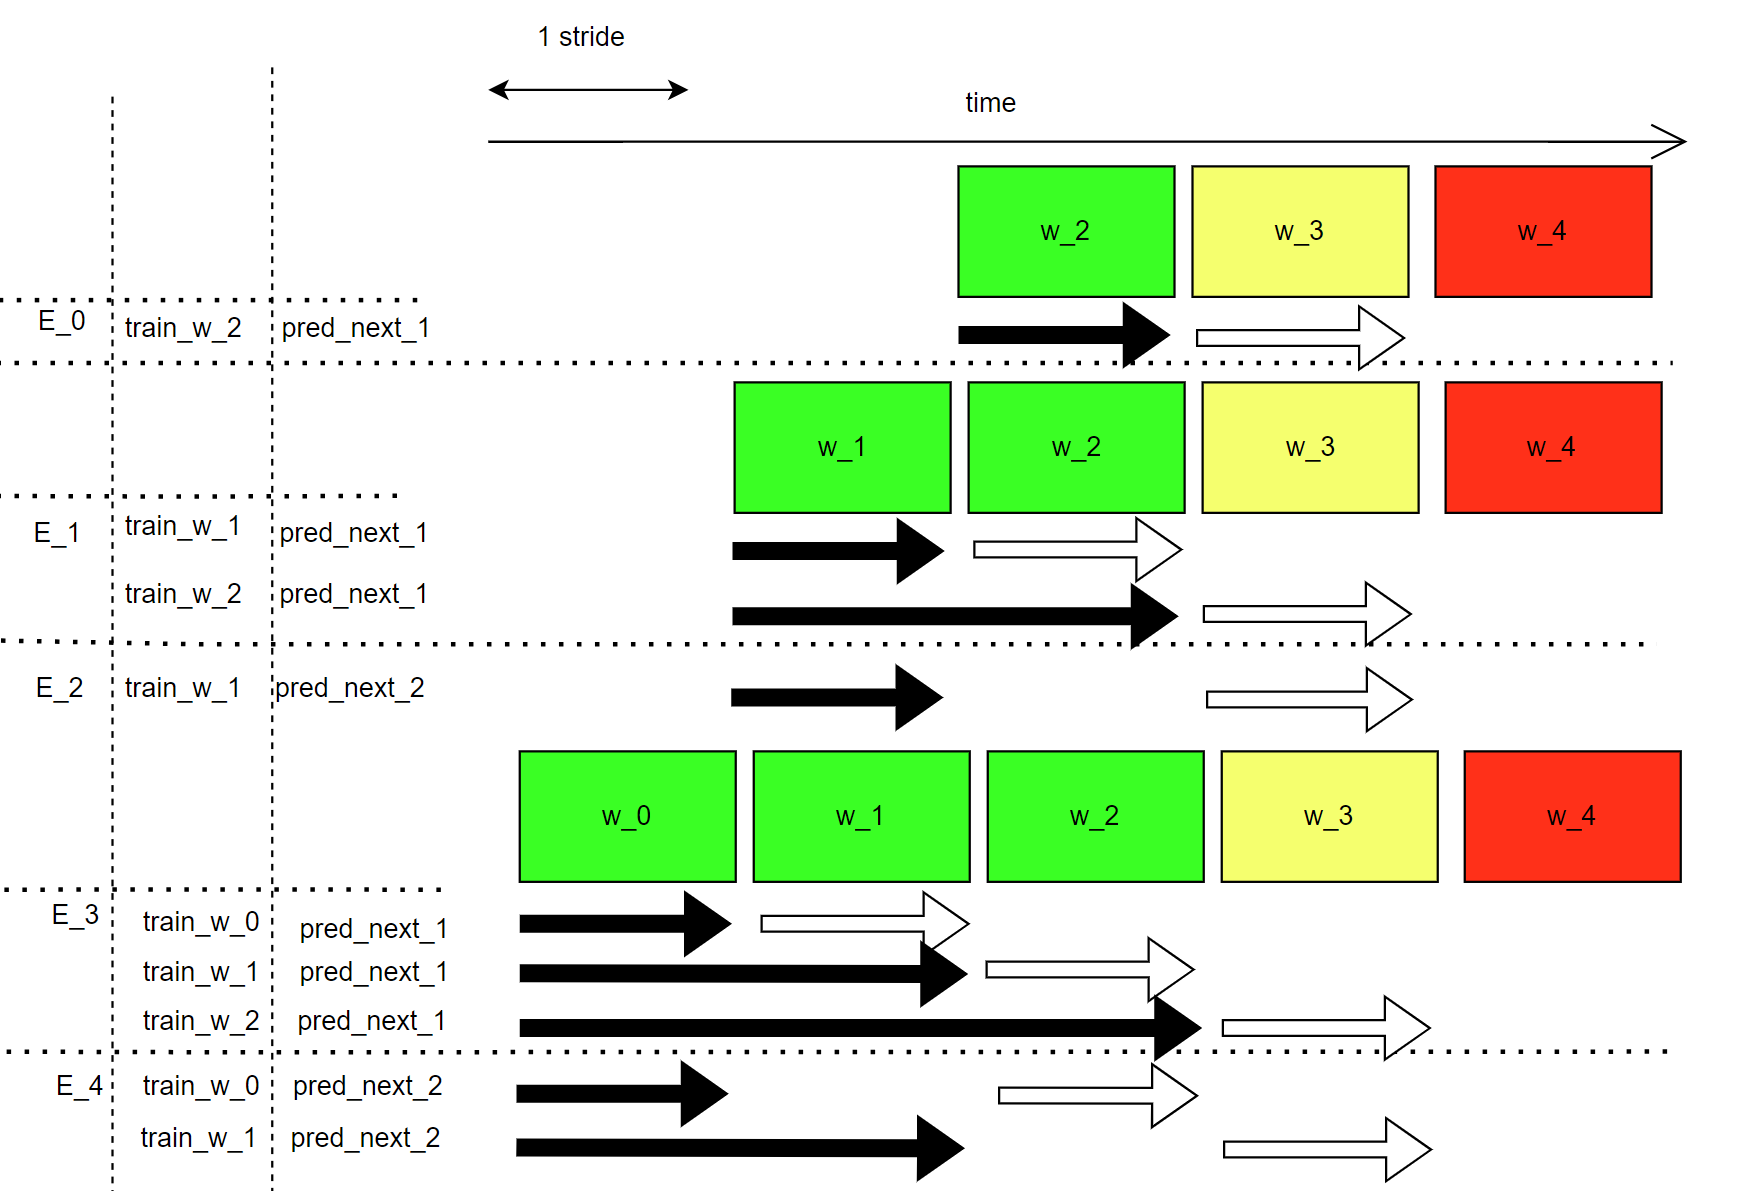
\includegraphics[width=.9\linewidth]{./images/screenshot_20220321_124235.png}
\caption{\label{window parameters}ensemble variation 1}
\end{figure}

\begin{figure}[htbp]
\centering
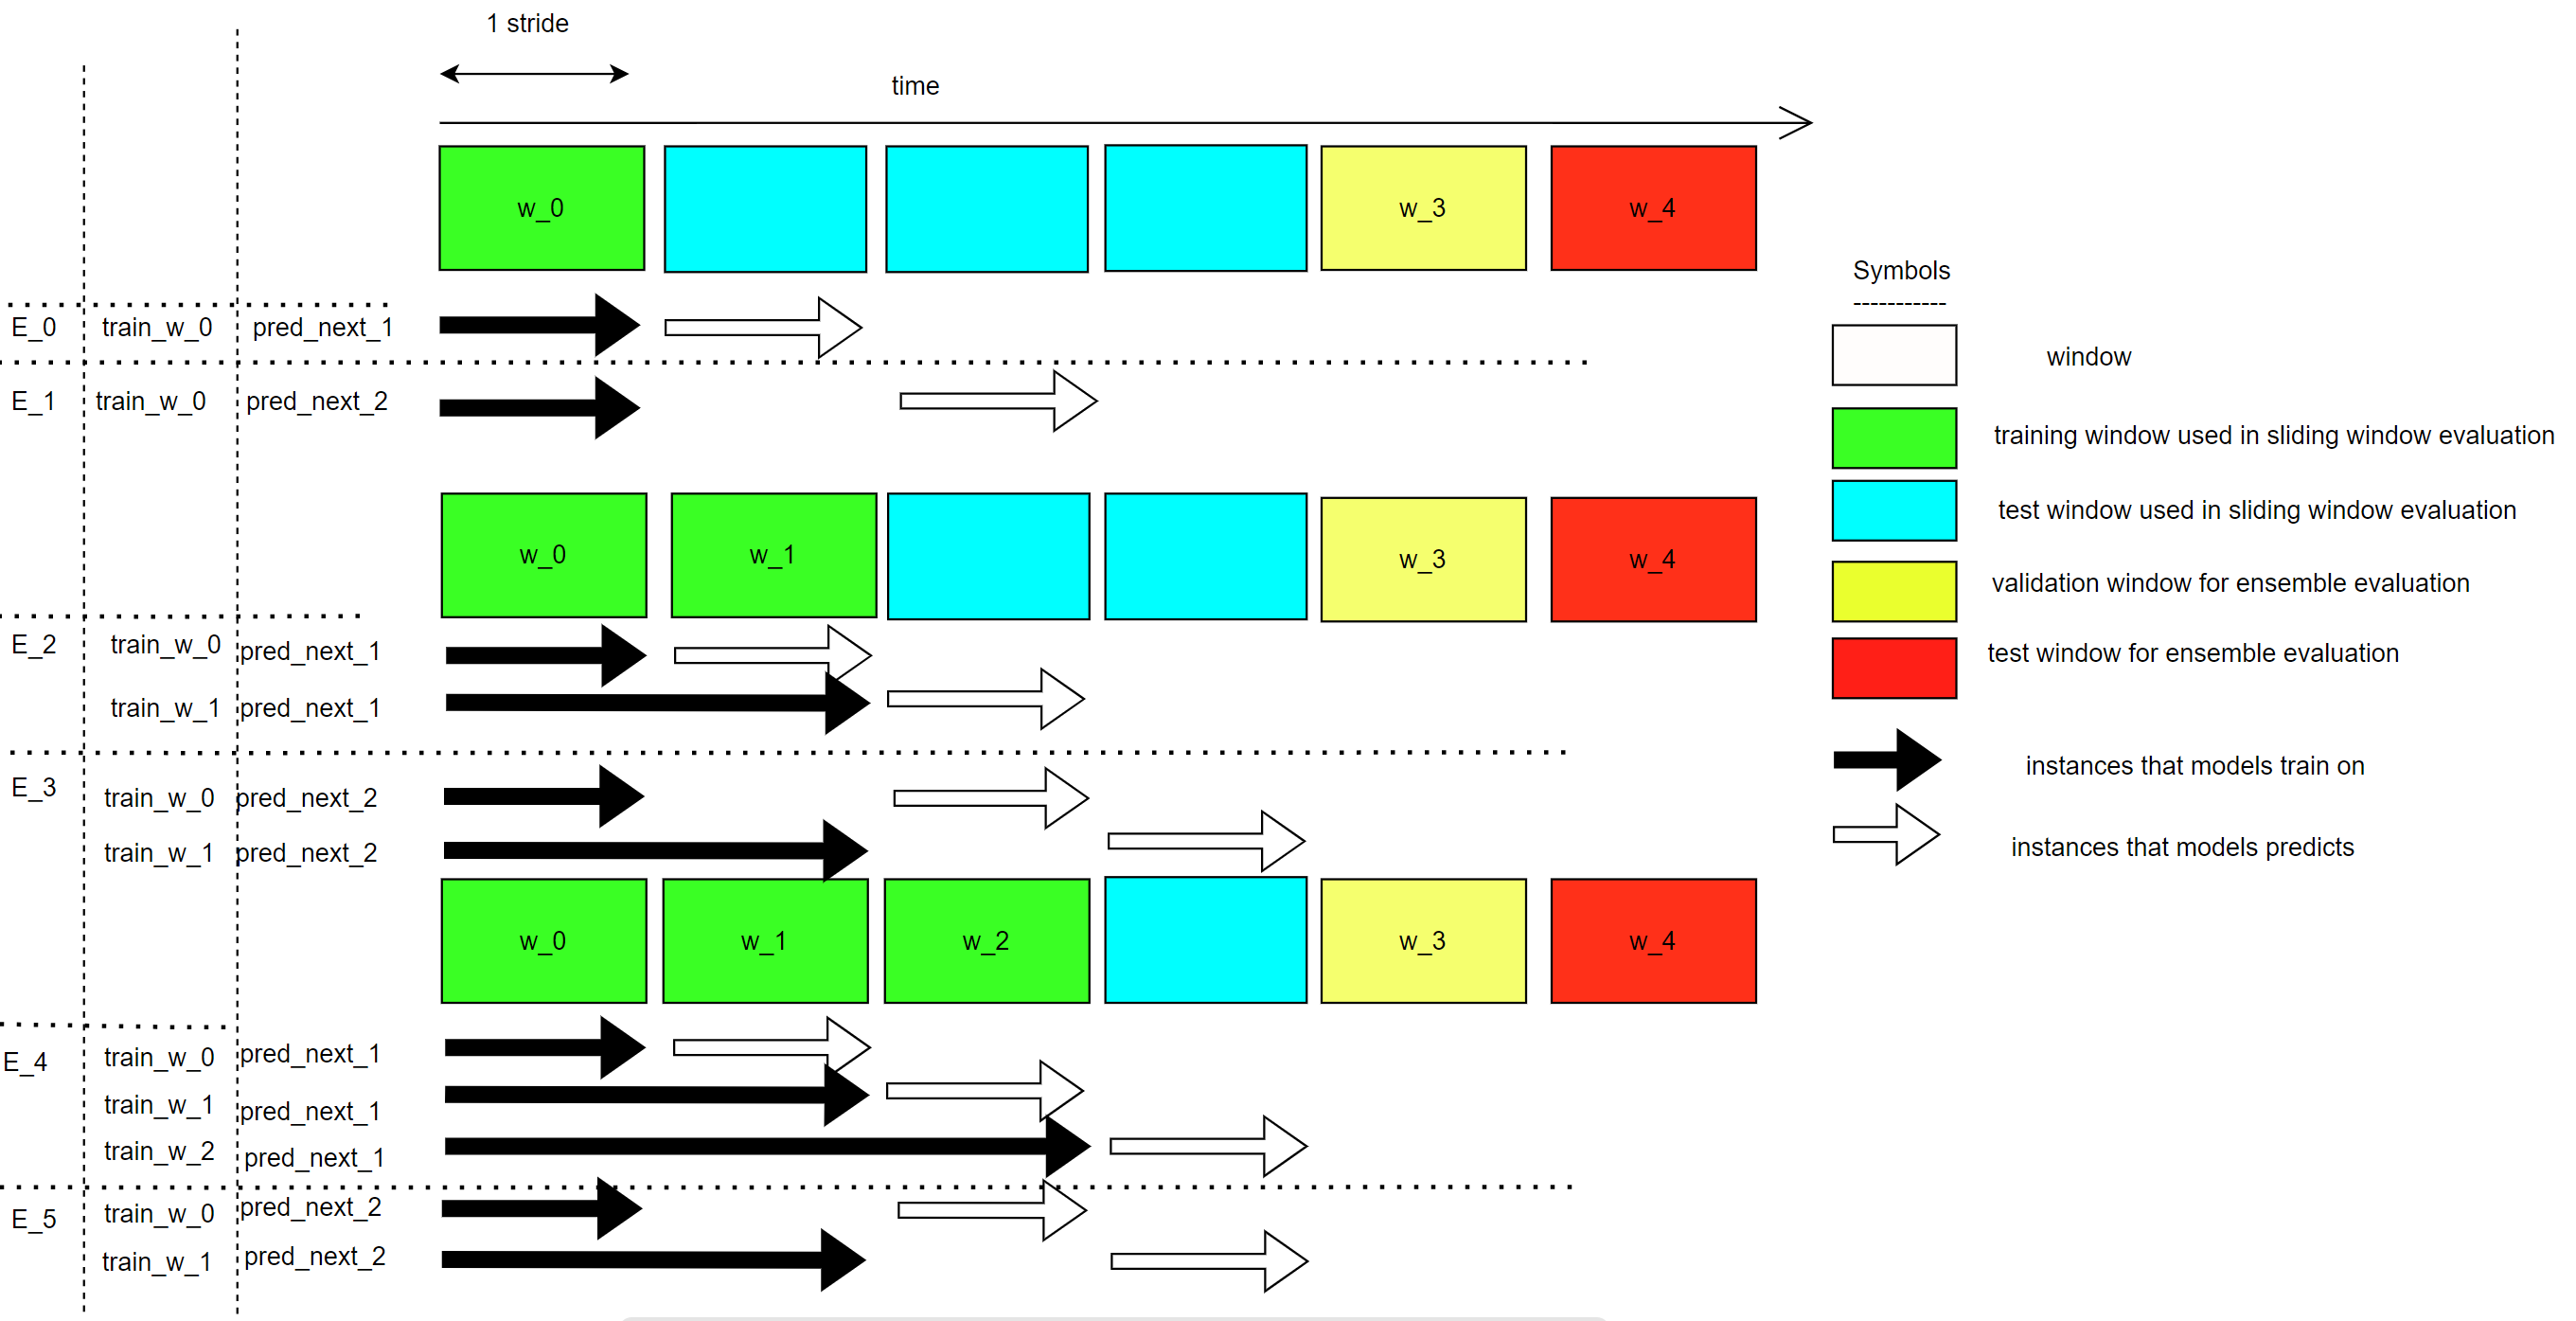
\includegraphics[width=.9\linewidth]{./images/screenshot_20220321_123955.png}
\caption{\label{window parameters}ensemble variation 2}
\end{figure}

In sliding window evaluation setting, one need to make sure proposed model and benchmark model is being tested as fair as possible. Furthermore, to extract the most benefit from ensemble models, participated models should provide diverse predictive information. Table \ref{parameters} provides list of parameters that must be considered to maximize diversity of predictive information in ensemble models.

According to \ref{parameters}, we categorize parameters of sliding window evaluation into four categories: windows parameters, temporal parameters, ensemble parameters, and granularity parameters.
Window parameters and ensemble parameters are self-explanatory, but granularity parameters and temporal parameters need clarification. Granularity is determined by prediction length during training. This parameter is important because it tells the model to minimize its mistake for certain time interval. In the other word, a model whose prediction performance is optimized over 10 days will be different to model whose performance is optimized over one day. Larger model that is trained on larger granularity ignores short term stochasticity of temporal dependencies.

It is important to note that temporal parameters can be applied ``during ensemble formation'' and ``in-between ensemble formation.'' During ensemble formation referring to the modeling step where, given a fix set of training length, N number of individuals are trained before voting predictive score to finalize an ensemble performance. In contrast, in-between ensemble formation occurs after ensemble performance of the previous timestep is finalized and set of training instance is adjusted before it will be used to train an ensemble model of the next time step.

In sliding window evaluation approach, there are a lot of combination of parameters that can effect model's predictive information. For this reason, one may consider using time budget to reduce size of solution space.

\section{Results}
\label{sec:org0bc802a}
\printbibliography
\end{document}
